
\section{Problem description}
% \begin{figure}
% \begin{center}
% 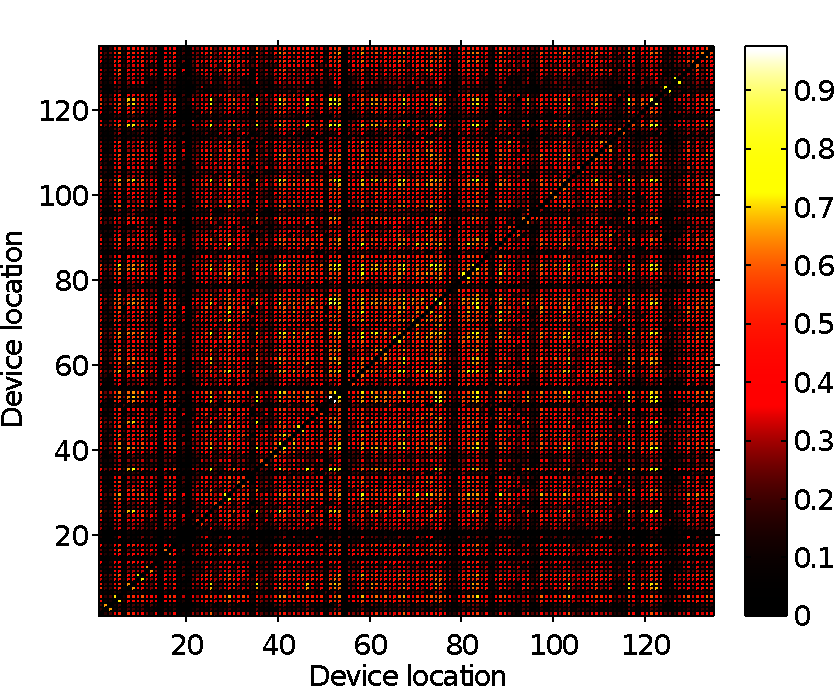
\includegraphics[width=.45\textwidth]{img/heatMap_raw_201106-eps-converted-to.pdf}
% \caption{Correlation coefficients of the raw traces from the Building 1 dataset (Section \ref{data:engbldg2}).
% The matrix is ordered such as the devices serving same/adjacent rooms are nearby in the matrix.}
% \label{fig:heatmap:raw}
% \end{center}
% \end{figure}

\begin{figure}[t!]
 \includegraphics[width=.5\textwidth]{img/estimator2.pdf}
 \caption{Two signals from HVAC pumps serving different rooms and different floors in the same building.}
 \label{fig:diagram1}
\end{figure}

The primary objective of SBS is to determine when multiple devices that are used (and not used) simultaneously.
The naive approach applies correlation analysis on raw data traces.  Figure~\ref{fig:diagram1} shows an example of 
two independent HVAC system power traces, serving different rooms on different floors.  Notice, they share a common diurnal power-draw
pattern, driven by occupancy in either room.  It is also driven by other factors, such as outside weather, temperature, incident light for
both rooms -- factors whose effect is captured by both systems.   
This trend is present in almost every trace and it hides 
the smaller fluctuations providing more specific patterns driven by local occupant activity.  
Such trends must be removed in order to uncover meaningful usage patterns between devices.

SBS is a signal processing and anomaly detection methodology that consists of the following step:

\begin{enumerate}
\item Decompose the signal into four frequency-range bins.
\item Construct a correlation matrix summarizing the inter-device usage patterns.
\item Repeat the process, comparing subsequent correlation matrices against the reference.
\end{enumerate}

Although SBS is great at narrowing down the search space, there is no way to address false-positive alarms and
has no notion of true-negatives and false-negatives.  Also, SBS does not use any building-specific semantic information
to diagnose problems.  This is, in part, its strength, because it can be applied to all buildings without prior knowledge
and yield valuable results, however, in order to use the results meaningfully in future studies, we need to 
get the signal names under a normalized set of descriptors and vocabulary.